
\tikzstyle{input_neuron}=[circle,draw=red!50,fill=orange!10,thick,minimum size=.2mm]
\tikzstyle{hidden_neuron}=[circle,draw=blue!50,fill=blue!10,thick,minimum size=1mm]
\tikzstyle{output_neuron}=[circle,draw=green!50,fill=green!20,thick,minimum size=1mm]
\tikzstyle{output}=[circle,draw=green!50,fill=green!20,thick,minimum size=1mm]
\tikzstyle{positive}=[circle,draw=red!50,fill=red!10,thick,minimum size=.2mm]
\tikzstyle{negative}=[circle,draw=blue!50,fill=blue!10,thick,minimum size=1mm]
\resizebox{6cm}{5cm}{%
	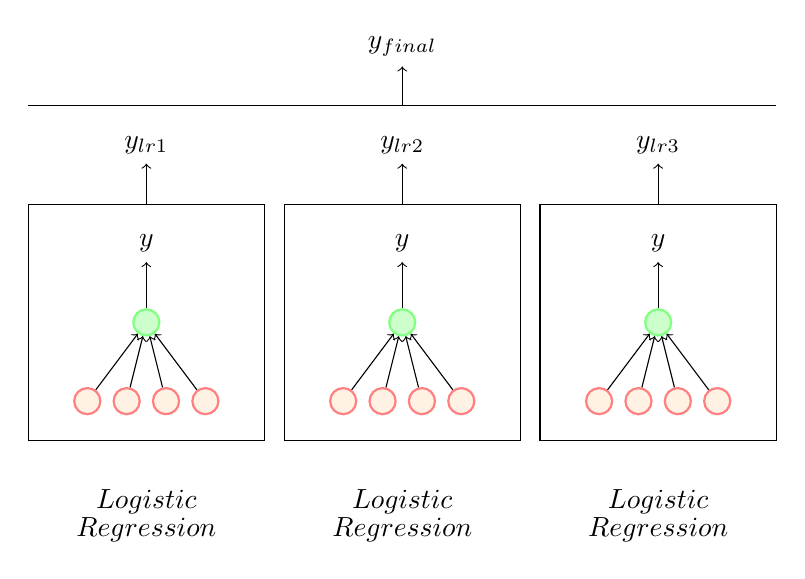
\begin{tikzpicture}
							
		\node [input_neuron] (in0) at (0.75,0.5) {};
		\node [input_neuron] (in1) at (1.25,0.5) {};
		\node [input_neuron] (in2) at (1.75,0.5) {} ;
		\node [input_neuron] (in3) at (2.25,0.5) {} ;
							
		\node [output_neuron] (out0) at (1.5,1.5)  {} ;
							
		\node (output0) at (1.5,2.5)  {$y$} ;
		\node (output1) at (1.5,3.75)  {$y_{lr1}$} ;
		\draw (0,0) rectangle  (3,3);
		\draw [->] (in0) -- (out0);
		\draw [->] (in1) -- (out0);
		\draw [->] (in2) -- (out0);
		\draw [->] (in3) -- (out0);
		\draw [->] (out0) -- (output0);
		\draw [->] (1.5,3) -- (output1);
						
							
		\node [input_neuron] (in4) at (4,0.5) {};
		\node [input_neuron] (in5) at (4.5,0.5) {};
		\node [input_neuron] (in6) at (5.0,0.5) {} ;
		\node [input_neuron] (in7) at (5.5,0.5) {} ;
							
		\node [output_neuron] (out1) at (4.75,1.5)  {} ;
							
		\node (output2) at (4.75,2.5)  {$y$} ;
		\node (output3) at (4.75,3.75)  {$y_{lr2}$} ;
		\draw (3.25,0) rectangle  (6.25,3);
		\draw [->] (in4) -- (out1);
		\draw [->] (in5) -- (out1);
		\draw [->] (in6) -- (out1);
		\draw [->] (in7) -- (out1);
		\draw [->] (out1) -- (output2);
		\draw [->] (4.75,3) -- (output3);
						
							
		\node [input_neuron] (in8) at (7.25,0.5) {};
		\node [input_neuron] (in9) at (7.75,0.5) {};
		\node [input_neuron] (in10) at (8.25,0.5) {} ;
		\node [input_neuron] (in11) at (8.75,0.5) {} ;
							
		\node [output_neuron] (out2) at (8,1.5)  {} ;
							
		\node (output4) at (8,2.5)  {$y$} ;
		\node (output5) at (8,3.75)  {$y_{lr3}$} ;
		\draw (6.5,0) rectangle (9.5,3);
		\draw [->] (in8) -- (out2);
		\draw [->] (in9) -- (out2);
		\draw [->] (in10) -- (out2);
		\draw [->] (in11) -- (out2);
		\draw [->] (out2) -- (output4);
		\draw [->] (8,3) -- (output5);
		\node [below] (head) at (4.75,-0.5)  {$Logistic$ } ;
		\node [below] (head) at (8,-0.5)  {$Logistic$ } ;
		\node [below] (head) at (1.5,-0.5)  {$Logistic$ } ;
		\node [below] (head) at (4.75,-0.85)  {$Regression$} ;
		\node [below] (head) at (8,-0.85)  { $Regression$} ;
		\node [below] (head) at (1.5,-0.85)  { $Regression$} ;
							
		\node (output3) at (4.75,5)  {$y_{final}$} ;
		\draw (0,4.25) -- (9.5,4.25);
		\draw [->] (4.75,4.25) -- (4.75,4.75);
	\end{tikzpicture}
}
